\documentclass[letterpaper]{article}

% Math packages
\usepackage{amsthm}
\usepackage{amsmath}
\usepackage{amssymb}

% For more complicated table formatting
\usepackage{multirow}
\usepackage{tabularx}
\newcolumntype{L}[1]{>{\raggedright\let\newline\\\arraybackslash\hspace{0pt}}m{#1}}
\newcolumntype{C}[1]{>{\centering\let\newline\\\arraybackslash\hspace{0pt}}m{#1}}
\newcolumntype{R}[1]{>{\raggedleft\let\newline\\\arraybackslash\hspace{0pt}}m{#1}}

% Remove line spaces between items of enumerate and itemize
\usepackage{enumitem}
\setlist{noitemsep}

% Adds double bracket symbols
\usepackage{stmaryrd}

% Allows to create negation symbols
\usepackage{MnSymbol}

% General math symbols
\DeclareMathOperator{\Id}{Id} % Identity function

% Theorem styles

%\renewcommand\thesubsection{\thesection.\Alph{subsection}}
%\renewcommand{\theequation}{\thechapter.\arabic{equation}}

\newtheorem{assump}{Assumption}
\renewcommand*{\theassump}{\Roman{assump}}

\newtheorem{axiom}[equation]{Axiom}
\newtheorem{defn}[equation]{Definition}
\newtheorem{prop}[equation]{Proposition}
\newtheorem{coro}[equation]{Corollary}
\newtheorem{thrm}[equation]{Theorem}

%\theoremstyle{definition}

\newenvironment{remark}{\emph{Remark}.}{}
\newenvironment{rationale}{\emph{Rationale}.}{\qed}
\newenvironment{justification}{\emph{Justification}.}{\qed}
\renewenvironment{proof}{\emph{Proof}.}{\qed}


% LOGIC symbols
% -------------

% Boolean symbols and algebra
\def\Bool{\mathbb{B}}
\def\TRUE{\textsc{true}}
\def\FALSE{\textsc{false}}
\def\AND{\wedge}
\def\bigAND{\bigwedge}
\def\OR{\vee}
\def\bigOR{\bigvee}
\def\NOT{\neg}

% Logical context and related symbols
\def\logCtx{\mathcal{S}}
\def\vstmtSet{\mathcal{S}_\textsf{v}}
\def\dstmtSet{\mathcal{S}_\textsf{d}}
\newcommand{\pAss}[1][\mathcal{S}] {\mathcal{A}_{#1}}
\DeclareMathOperator{\truth}{truth}

% Experimental test symbols
\newcommand{\exptSet}{\mathcal{E}}
\newcommand{\expt}[1][e] {\mathsf{#1}}
\DeclareMathOperator{\result}{result}
\def\SUCCESS{\textsc{success}}
\def\FAILURE{\textsc{failure}}
\def\UNDEF{\textsc{undefined}}

% Statements
\def\tautology{\top} % Tautology
\def\contradiction{\bot} % Contradiction
\newcommand{\stmt}[1][s] {\mathsf{#1}} % Statement
\newcommand{\tstmt}[1][s] {\bar{\mathsf{#1}}} % Theoretical statement

% Relationships between statements
\def\comp{\doublefrown} % Compatibility
\def\ncomp{\ndoublefrown} 
\def\narrower{\preccurlyeq} % Narrowness
\def\nnarrower{\npreccurlyeq}
\def\snarrower{\prec}
\def\nsnarrower{\nprec}
\def\broader{\succcurlyeq} % Broadness
\def\nbroader{\nsucccurlyeq}
\def\sbroader{\succ}
\def\nsbroader{\nsucc}
\def\indep{\upmodels} % Independent
\def\nindep{\nupmodels}

% Experimental domains and related symbols
\newcommand{\edomain}[1][D] {\mathcal{#1}} % Experimental domain
\newcommand{\tdomain}[1][D] {\bar{\mathcal{#1}}} % Theoretical domain
\newcommand{\basis}[1][B] {\mathcal{#1}} % Basis
\newcommand{\resPoss}[1][x] {\mathring{#1}} % Residual possibility
\newcommand{\estPoss}[1][x] {\dot{#1}} % Established possibility

% Formatting for experimental relationships
\newcommand{\erel}[1][r] {#1}

% Formatting for sentence statements
\newcommand{\statement}[1] {\emph{``#1"}}

% Formatting for reference
\newcommand{\refStmt}[1][r]{\textbf{#1}}

\DeclareMathOperator{\ver}{ver}
\DeclareMathOperator{\fal}{fal}
\DeclareMathOperator{\und}{und}

\DeclareMathOperator{\interior}{int}
\DeclareMathOperator{\exterior}{ext}

% Level of detail
\def\eqgran{\doteq}
\def\finer{\leqdot}
\def\nfiner{\nleqdot}
\def\coarser{\geqdot}
\def\sfiner{\lessdot}
\def\scoarser{\gtrdot}


\usepackage{tikz}

% Remove line spaces between items of enumerate and itemize
\usepackage{enumitem}
\setlist{noitemsep}

\begin{document}

\title{A Refactoring - new attempt}


\author{Gabriele Carcassi}
%\email{carcassi@umich.edu}
\author{Christine A. Aidala}
%\affiliation{
%	Physics Department \\
%	University of Michigan \\
%	Ann Arbor, MI 48109 \\
%}

\date{\today}

\begin{abstract}
	We lay the groundwork for a formal framework that studies scientific theories and can serve as a unified foundation for the different theories within physics. We define a scientific theory as a set of verifiable statements, assertions that can be shown to be true with an experimental test in finite time. By studying the algebra of such objects, we show that verifiability already provides severe constraints. In particular, it requires that a set of physically distinguishable cases is naturally equipped with the mathematical structures (i.e. second-countable Kolmogorov topologies and $\sigma$-algebras) that form the foundation of manifold theory, differential geometry, measure theory, probability theory and all the major branches of mathematics currently used in physics. This gives a clear physical meaning to those mathematical structures and provides a strong justification for their use in science. Most importantly it provides a formal framework to incorporate additional assumptions and constrain the search space for new physical theories.
\end{abstract}

\maketitle

%\linenumbers

\section{Introduction}

When considering physics as a discipline, one cannot help but notice that it is essentially composed of different theories and models loosely connected to each other, each with its own starting points and realm of applicability. Classical mechanics, electromagnetism, general relativity, quantum mechanics, thermodynamics and so on may share some general ideas but, in the end, they all have their own separate foundation, either in a different set of laws and principles or simply in positing a unique mathematical structure. This state of affairs is so entrenched in our field it somehow feels like the proper, if not the only, approach. But is it? Or does this approach actually hinder progress and understanding?

We can gain perspective by comparing to different fields of science and engineering. For example, in computer science theory one starts by defining symbolic languages and computational devices~\cite{Turing} and then shows that no algorithm exists that can correctly decide whether an arbitrary program terminates given an arbitrary input~\cite{Sipser}. In communication theory one defines channels and the information they carry~\cite{Shannon} and proves general results such as calculating the maximum rate at which information can be transmitted over a channel given a set amount of noise~\cite{Pierce}. In control theory one defines a system in terms of state, inputs and outputs~\cite{Brogan} and then looks for general strategies for control such as Kalman filtering~\cite{Kalman}. These theories, with their respective mathematical structures and results, are \emph{general} in the sense that they apply to all control systems, all communication systems and all computational devices. More specific topics in each field are constructed by further constraining those general mathematical structures. In other words, the subject matter has been properly defined formally and therefore the results follow simply from the mere definition of the problem.

In physics there is no equivalent. Classical mechanics, thermodynamics and quantum mechanics are not specific topics within some more general formal theory. But how would that work? As in the other general theories, we need to clarify what our starting points are and let the logic follow. The first requirement of a physical theory, or rather of any scientific theory in general, is that it is experimentally testable. So we would start by characterizing the properties and limitations of experimental verification. The second requirement, which is where physics starts, is identifying states and processes. After those are characterized in general, we can then specialize them for different cases. Some processes will be deterministic and reversible. Some processes will be non-deterministic and some will have equilibria. Some states can be broken into parts and some cannot. By adding different assumptions on states and processes we would recover classical Hamiltonian mechanics in one case, quantum mechanics in another and thermodynamics in yet another. In all these theories, some basic properties will be common simply because states need to be identified experimentally, and some properties will be different because the type of state or the type of process is different. This is what we mean by a general mathematical theory of experimental science.

%[rectangle, draw, fill=black!10, inner sep=5pt, text width=4cm, text badly centered, minimum height=1.2cm]
%every node/.style={draw, align = center},

\begin{figure}\label{twoQuestions}
	\centering
	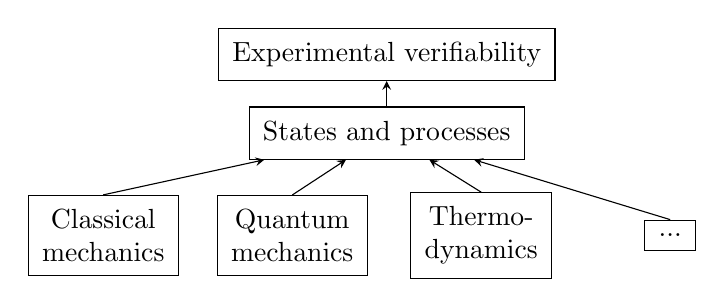
\begin{tikzpicture}
	[child anchor = north, every node/.style={draw, align = center, inner sep=5pt},
	edge from parent/.style={draw, ->, -latex, stealth-},
	level 1/.style={level distance=1cm},
	level 2/.style={level distance=1.3cm, sibling distance=2.4cm}, sloped]
	\node {Experimental verifiability}
	child {node {States and processes}
		child {
			node {Classical \\ mechanics}
		}
		child {
			node {Quantum \\ mechanics}
		}
		child {
			node {Thermo- \\dynamics}
		}
		child {
			node {...}
		}
	};
	\end{tikzpicture}
	\caption{Overall structure for a general mathematical theory of experimental science. The starting point is experimental verification. States and processes are particular types of experimentally testable objects. Different theories in physics describe particular states under particular processes.}
\end{figure}

Such a general theory would force us to clarify our assumptions, thus the realm of applicability of each theory. It would always put physics at the center of our discussion, as physical ideas are the starting point for our formal framework and not after-the-fact interpretations. It would give science sturdier mathematical grounds, as each mathematical symbol is given a precise meaning and non-physical objects are excluded by construction. It would foster connections between different fields of knowledge: nature does not care about such divisions. It would provide a framework in which to pose new questions and solve old ones. In other words: it would provide a better foundation for physics and for the rest of the sciences. Developing a general mathematical theory for experimental science could be compared to what happened in mathematics during the first half of the last century, when it was reorganized using logic and set theory as its foundation, which had profound repercussions in the field. Our preliminary work in both physics~\cite{Carc1} and math~\cite{Carc2} convinced us that such a goal is possible and within reach.

The aim of the present work is to lay down the beginning of a general mathematical theory of experimental science, limited to the part concerning experimental verification. We start by defining verifiable statements: assertions whose truth can be verified experimentally in finite time. We study the logic of these statements, which is different from the standard Boolean logic because of finite time termination. We define experimental domains as a collection of verifiable statements that, if given an indefinite amount of time, we can keep testing, forever refining our knowledge. From each experimental domain we construct its possibilities: the different cases we can experimentally distinguish. The main result is that \textbf{each set of experimentally distinguishable possibilities comes equipped with a natural second-countable Kolmogorov topology, where each open set corresponds to a verifiable statement, and a natural $\sigma$-algebra, where each Borel set corresponds to a theoretical statement which gives predictions for verifiable ones.} For example, \statement{the mass of the particle is more than $0.4$ and less than $0.6$ MeV} is a verifiable statement precisely because $(0.4, 0.6)$ is an open set, while \statement{the mass of the particle is exactly $0.5$ MeV} is not verifiable because $[0.5,0.5]$ is not an open set.\footnote{The standard topology of the real numbers keeps track of finite precision measurements.} From that general result we can derive the following conclusion: \textbf{any set of physically distinguishable cases has at most cardinality of the continuum}. That is, the only thing we can do to distinguish a particular case is run the tests for a countable set of statements, the output of which can be imagined as a countable sequence of true and false. This is equivalent to the binary representation of a real number. In a nutshell, \textbf{experimental verification by itself guarantees us the existence of two mathematical structures that are the foundations of most tools used in physics}, such as differential geometry (Riemannian and symplectic), measure theory, probability theory and many others.

%In this paper we briefly present the starting point for our general mathematical theory of experimental science. It is the product of a decade spent in reverse engineering the laws of particle mechanics~\cite{Carc1} and our subsequent work on formalizing the starting points~\cite{Carc2}. Our overall program is large and ambitious and a journal article cannot treat it comprehensively. Therefore we will only present an overview of the basic concepts, which are already well consolidated and provide a good template to understand our approach. We will only provide a sketch for the proofs, which can be found in the draft of our open access book~\cite{Carc3} together with more details, discussions and insights.

While this result is remarkable by itself, the most interesting aspect is that it can be used as a cornerstone for a more general theory. Conceptually, in the same way that topological spaces keep track of what can be verified experimentally, manifolds keep track of objects that can be identified by continuous quantities, differentiable manifolds keep track of objects that allow a density to be defined over them and symplectic manifolds (i.e. phase space of classical mechanics) allow the density to be coordinate invariant (i.e. observer independent). By doing all this work formally we will be forced to recognize the assumptions that go into those structures, and understand if and how they fail. For example, we are currently in the process of identifying the necessary and sufficient conditions such that a set of verifiable statements defines a continuous quantity. While, as one would expect, these can only correspond to an idealized case where one pretends a better precision measurement can always be achieved, they also tell us precisely how this idealized case fails which can be relevant to work on Planck scale physics. But whatever other tools we will have in that case, we \emph{know} we will always have at least a topology and a $\sigma$-algebra.

As another example, note that the set of discontinuous functions from $\mathbb{R}$ to $\mathbb{R}$ has cardinality greater than the continuum and therefore cannot represent a set of physically distinguishable objects. This means that the square integrable space of functions typically used in quantum mechanics is far too big, and, in fact, it contains unphysical elements, such as states with infinite energy. However, the Schwartz space, like the set of continuous functions, has cardinality of the continuum and can be given a second-countable Kolmogorov topology.\footnote{It also has other properties that map to physical requirements. For example, quantities of the form \unexpanded{$\langle \psi|Q^n P^m|\psi\rangle$} are always finite and the Fourier transform is always well defined.} To our understanding, the reason why Hilbert spaces are mathematically useful is because one can take limits and use the vector space norm to converge. However, we may instead be able to use the corresponding $\sigma$-algebra to take limits, like one does in probability and measure theory. In other words, we may be able to construct, within this framework, a more mathematically sound and physically motivated foundation for quantum mechanics that includes the objects and only the objects that are physically meaningful.

As a last example, we also believe we can form a connection to computer science. We can characterize the output of a computational device as a set of verifiable statements (e.g. \statement{the third bit of output is 1}) that are a function of the input, which can also be characterized as verifiable statements (e.g. \statement{the second bit of the input is 0}). In this context, all possible inputs form the possibilities of our space, as they define all possible outputs of the computation. Now suppose we have a function from the input to a Boolean value. Then we can write the statements \statement{the input is such that the output of the function is true} and \statement{the input is such that the output of the function is false}. If both these statements correspond to open sets on the possible inputs then they are verifiable statements and we construct a test (i.e. a program) that will always terminate. That is, we can combine tools from topology and computer science to answer a question of the type: is this scientific problem testable or computable? In a similar way, connections to information theory can also be established: a deterministic and reversible process, in fact, is one for which description of the input is equivalent to the description of the output, which means information entropy is conserved. These links illustrate the potential as a theory of experimental science, and not just physics.

We hope that it is clear by now that a general mathematical theory of experimental science is missing, is possible and would be extremely useful. Whether you work on condensed matter, quantum thermodynamics, complex systems, particle physics, gravitation or grand unified theories, if what you are doing is science you will have, at some point, experimental verification. You will have problems (often the most interesting ones) that arise from questions such as: what is it that I can measure? How do I do it? Under what assumptions do the quantities in my theory map to those measurements? When are they even well defined? What can I compute within my theory? What is testable? Currently, you do not have a general framework to pose those questions. And it turns out you do not need a completely ad-hoc one for your specific field. The mere \emph{logic} of experimental verification requires a particular structure. And there is a lot more to experimental verification than its logic: the quantity itself has to, at least in a sense, exist over a finite period of time to be measurable, there must exist a process to transfer that information to a measurement device, the system cannot be assumed to be always completely isolated as it would not be physically accessible. If you are working on foundational aspects, chances are you may already be thinking about some of these issues as they relate to your field. But what parts of those problems are specific to your field? How much can be treated generally, so that not only each field has less work to do but also we have a common language across fields? What are the assumptions specific to your field and those that are more general? A general mathematical theory of experimental science would provide you with a formal framework to precisely pose and possibly answer those questions. As the starting points are clarified, the foundations of different fields may be affected, or even partially integrated, and potentially change how they are taught as well.

The irony is that while the project is extremely ambitious, the biggest obstacles are not, at this point, technical. The biggest obstacles are sociological. On one side the nature of this work is extremely interdisciplinary. On the other side math and physics are divided into fields and sub-fields that are increasingly narrow.\footnote{We attended a topology conference where there seemed to be a disconnect between what mathematicians and condensed matter physicists meant by topology, to the point that they frequently talked past each other.} This means that this work does not fit naturally within any community while requiring technical expertise from many. To obviate these problems, borrowing practices from the open source software community, we are developing our main body of work in the open~\cite{Carc3}, so that we can address the topic in its entirety, and our colleagues in philosophy, mathematics and physics can all check their respective parts. This article is the product of that process and focuses on current results of greater interest to physicists, omitting more mathematical and philosophical details that can be found in the broader work.

\section{A standard for precision?}

Mathematics has evolved a set of rules and standards for what constitutes a well-posed mathematical theory. There is no such standard in science in general and in physics in particular. In fact, given that some fields are mostly driven by data and heuristics while others are driven by mathematical formalism, we have found divergent opinions in what can and should be formalized. We therefore had to develop our own standard, which is based upon the following insights.

\textit{Formal systems cannot fully capture scientific theories.} The same mathematical structure (e.g. the equation $a= bc$) can refer to multiple physical relationships (e.g. Newton's second law or Ohm's law) which cannot be reconstructed solely on the basis of the formal relationships. Moreover, qualitative reasoning in many fields can be carried out independently. In this light, formal systems are a poor starting point for a scientific theory.

\textit{Formal systems in science should be justified, not interpreted.} We want to start from the informal definitions of the physical objects, be clear as to what aspects are formalized and why that formalization follows. The formal system, then, is a tool useful to check for consistency and clarification of particular aspects of the theory. It is useful only insofar its connection to the physical content is clear.

Our framework will therefore consist of both informal and formal parts. We distinguish two ways new concepts are introduced: axioms and definitions. \textbf{Axioms} introduce new elements: they define new concepts and what aspects are captured in the formal system.  \textbf{Definitions} further characterize already introduced objects, without introducing new elements in the formal system. Both axioms and definitions will consist of two parts. The first gives the intuitive, informal description while the second gives the formal characterization. The formal part will necessarily not capture the entirety of the informal concept. Where needed, a \textbf{justification} will accompany axioms and definitions. These are informal arguments that explain why the formal objects must have those formal properties. All \textbf{propositions} and \textbf{theorems} are declared and proven in the formal system, and they deal with objects that are now both mathematically and scientifically well specified.

The overall goal is to keep the axioms to a minimum and to a level of simplicity that is easily checked. This minimizes the part of the framework that can potentially be open to inconsistencies.

Axioms, definitions and justifications are included in the mathematical section, with the rest of the formal elements. They should be seen as integral part of the framework.

\section{Basic formal structures?}

The starting point of our framework is the \textbf{principle of scientific objectivity} which states \statement{Science is universal, non-contradictory and evidence based}. Every physical theory, then, must give us a set of logically sound statements linked with some notion of experimental verification. The content of the statements, what can be verified and how, will vary from theory to theory, but logical consistency and verifiability must be common to all of them. Therefore we will have two set of axioms: the \textbf{logical consistency axioms} and the \textbf{experimental verifiability axioms}. We start with the first set.

\subsection{Logical consistency}

The \textbf{axiom of context} establishes that \textbf{statements} are organized into \textbf{logical contexts}. It is the context that defines their meaning and logical relationships. The definition of a physical object, for example, may change depending on our goal: if we measure the mass of the electron, its value is assumed to be unknown; if we perform particle identification in a detector, the mass of the electron is assumed to be a particular value. Each context has to be such that the meaning of each statement has no ambiguity and therefore it is associated with a single, well-defined truth value. This is, in general, not known: it cannot be proven or deduced. Ultimately, it is the role of experimentation to find it.

The \textbf{axiom of possibility} establishes that not all truth assignments are consistent with the meaning of the statements. For example, it is not possible for \statement{the particle is an electron} and \statement{the particle is a positron} to be true at the same time. As the context must fully specify the meaning of each statement, all these relationships must be well-specified. A context therefore will define the \textbf{possible assignments} for all statements, and the actual truth must be one of them.

Lastly, the \textbf{axiom of closure} establishes that we can always find a statement whose truth depends on the truth of others through a chosen Boolean function. For example, we can find the negation of a statement, the conjunction (logical AND) of any two statements, and so on.

These three axioms introduce the basis of a logic system all scientific theories must adhere to. We can visualize a logical context as a table. Suppose we have a context $\logCtx$ which contains at least the following statements:
\begin{description}
	\item $\stmt_1=$\statement{that animal is an animal}
	\item $\stmt_2=$\statement{that animal is a cat}
	\item $\stmt_3=$\statement{that animal is a mammal}
	\item $\stmt_4=$\statement{that animal has three bones in the middle ear}
	\item $\stmt_5=$\statement{that animal is a dog}
	\item $\stmt_6=$\statement{that animal is black}
	\item $\stmt_7=$\statement{that animal is a plant}
\end{description}
We would have:
\begin{center}
	\begin{tabular}{c|c|c|c|c|c|c|c}
		$\stmt_1$ & $\stmt_2$ & $\stmt_3$ & $\stmt_4$ & $\stmt_5$ & $\stmt_6$ & $\stmt_7$ & ... \\
		\hline
		T & T & T & T & F & T & F & ... \\
		T & T & T & T & F & F & F & ... \\
		T & F & T & T & F & T & F & ... \\
		T & F & F & F & T & T & F & ... \\
		T & F & F & F & F & F & F & ... \\
		... & ... & ... & ... & ... & ... & ... \\
	\end{tabular}
\end{center}
where each line represents a possible assignment, each column a statement and each cell the truth value for each statement under the given assignment.

We can give some further definitions, which we introduce with examples based on the previous table. We say $\stmt_3$ and $\stmt_4$ are \textbf{equivalent}, noted $\stmt_3 \equiv \stmt_4$ because they have the same truth value in each assignment (only mammals have three bones in the middle ear). We say $\stmt_2$ is \textbf{narrower} than $\stmt_3$ (i.e. more specific), noted $\stmt_2 \narrower \stmt_3$, because whether the first one is true the second one is true as well (if the animal is a cat, it is also a mammal). We say $\stmt_2$ and $\stmt_5$ are not \textbf{compatible}, noted $\stmt_2 \ncomp \stmt_5$, because there is no assignment in which they are both true (if the animal is a cat, it is not a dog). We say $\stmt_2$ is independent from $\stmt_6$, noted $\stmt_2 \indep \stmt_6$, because the truth value of one does not constrain the truth value of the other (knowing whether the animal is a cat or not does not tell us whether it is black or not). We say $\stmt_1$ is a \textbf{tautology} $\tautology$, noted $\stmt_1 \equiv \tautology$, because it is true in every assignment. We say $\stmt_7$ is a \textbf{contradiction} $\contradiction$, noted $\stmt_7 \equiv \contradiction$, because it is false in every assignment. All others are \textbf{contingent}.

From now on, we will not differentiate between two statements that are equivalent. That is, we will implicitly refer to the equivalence classes. With that in mind, one can show that a logical context is a \textbf{complete Boolean algebra} and that $\narrower$ is a partial order, the one corresponding to the lattice of the algebra. While this should not be surprising, the point is that we start from premises that are easily justified and that give a clear understanding of what the formal object represents.

This will be essential when adding new definitions. Any other formal structure imposed on the statements, in fact, is capturing other properties of the same objects and will have to ``play nice'' with the above logical structure. This means that the notion of equivalence will, in practice, become an isomorphism within the new structure; the ordering imposed by numeric quantities will be a specialized version of the one imposed by $\narrower$; the notion of independence will relate to the notion of independence in statistic, probability, linear algebra, dynamical system, and so on. Understanding this simple logical structure, then, means getting insights in many different areas and in how they are ultimately connected.

% In mathematical logic, this is typically a well formed formula. This cannot work for us: what we are interested in is the meaning of the assertion and not how it is expressed. For example, \statement{this animal is a dog} and \statement{questo animale \`e un cane} represent the same fact expressed in different languages. As science is universal, it should not matter the language, units or reference system used to make an assertion.\footnote{In the same vein, a statement is not necessarily one sentence as it has to include all the information needed to understand what exactly we are talking about. These are the type of philosophical issues that are discussed at greater length in~\cite{Carc3}.} While we will still use standard mathematics for the formal system, we introduce a variation of algebraic logic to represent our ``informal'' assertions. We start by defining our truth bearer as:

%Note how the first part of the definition captures the informal meaning of what we are describing, while the second part captures the part that is formalized. This pattern will be present in most of our definitions and it serves to clarify both what is being formalized and how. Therefore, in science, the statement is an assertion while for the math it is just an element in some set.


%Note that the possible assignments are just hypotheticals. They are not actual physical entities. There is only one truth value, the one found experimentally. Logical consistency is defined on the truth assignments and not on the truth values. This allows us, for example, to track whether the meaning of each statement allows it to be true or not.

%This system not only allows us to use formal classical logic while keeping the statements informal, but is also equipped to capture causal relationships.\footnote{Note that the axioms prevent any form of paradox, simply because a possible assignment must exist. Therefore situations like \statement{this statement is not true} are ruled out simply because they cannot satisfy the axioms.} For example, $\stmt_1=$\statement{the thermometer indicator is between 24 C and 25 C} and $\stmt_2=$\statement{the temperature is between 24 C and 25 C} are equivalent because one is true if and only if the other is true (on the assumption that our thermometer is actually working). We can also define other semantic relationships.


\subsection{Experimental verifiability}

Having seen the logical consistency axioms, we turn our attention to the experimental verifiability axioms.

The \textbf{axiom of verifiability} establishes that some statement are experimentally \textbf{verifiable}, meaning we have a test at our disposal that, if the statement is true, will terminate successfully in finite time. If the statement is not true, the test may terminate unsuccessfully or never terminate. To give an example, consider the following:
\begin{enumerate}
	\item find a swan
	\item if it is black terminate successfully
	\item go to step 1
\end{enumerate}
This will terminate if a black swan is found, but it will not terminate if no black swans exist (i.e. absence of evidence is not evidence of absence). The axiom also states that tautologies and contradictions are verifiables (i.e. they can be associated with trivial tests) and that if one statement is equivalent to a verifiable one, then it is also verifiable (i.e. we can use the test of the second since either both statements are true or both are false).

Termination in finite time is important as it imposes a different logical structure.\footnote{This is broadly recognized in computer science theory and in constructive logic.} Because of non-termination, failure to verify is not verification of the negation. That is, the negation of a verifiable statement is not necessarily a verifiable statement.

The \textbf{axiom of finite conjunction verifiability} establishes that, given a finite set of statements, we can verify their conjunction (i.e. the logical AND). In fact, we can execute one test at a time, and if they are all successful, they will be so in finite time therefore the conjunction will be verified as well. This will not extend to the infinite case.

The \textbf{axiom of countable disjunction verifiability} establishes that, given a countable set of statements, we can verify their disjunction (i.e. the logical OR). In fact, if the disjunction is true then one statement must be true. Once that is verified, we can terminate regardless of how many other statements are there in the disjunction. The set of statements must be countable, though, or it may take infinite time to find the statement that is true.

On top of these axioms we can define \textbf{decidable statements} as the ones that can be both verified and falsified experimentally (i.e. their negation is a verifiable statement). One can prove that the finite disjunction and the finite conjunction of decidable statements is also decidable.

We therefore have three types of algebras embedded one into the other. The logical context $\logCtx$ is a complete Boolean algebra; the set of all verifiable statement $\vstmtSet \subset \logCtx$ is, in general, not a Boolean algebra but a complete Heyting algebra; the set of all decidable statements $\dstmtSet \subset \vstmtSet \subset \logCtx$ is a (finite) Boolean algebra. The interplay between these structures is important and leads to topologies and $\sigma$-algebras, the foundations for geometry, Lie algebras, measure theory, probability theory and most of the mathematical structures widely used in physics.

\subsection{Domains and possibilities?}

Finite time termination not only imposes a different logical structure, but it also limits the number of statements that can be verified. Even when given an arbitrarily long time, a countable set of statements is the most that can be verified. However, due to the logical relationship between statements, one does not need to test all of them: if \statement{the mass of the photon is less than $10^{-6}$ eV} is experimentally verified, there is no need to test whether \statement{the mass of the photon is greater than $10^{-6}$ eV}.

Given a set $\edomain$ of verifiable statements, we call a \textbf{basis} $\basis \subset \edomain$ a subset whose tests are enough to verify the whole set. Formally, $\edomain$ can be generated from $\basis$ using finite conjunction and countable disjunction. We say $\edomain$ is an \textbf{experimental domain} if it is a maximal set (i.e. includes all the verifiable statements) generated from a countable basis.

An experimental domain represents all experimental evidence that can be acquired in an indefinite amount of time. It represents the most fundamental object in our framework and, if our scientific theory is evidence based, it must be fully specified by an experimental domain.

Not all statements in a scientific theory, though, are verifiable statement. For example, \statement{there is no extra-terrestrial life} is not something we can verified (at best we can only conclude we have found none where we looked), and neither is \statement{the mass of the photon is exactly 0 eV} (at best we can exclude is above a certain threshold). In general, while negations are not necessarily verifiable, we can still logically talk about them and they must be included in our theory.

Given an experimental domain $\edomain$ we define its \textbf{theoretical domain} $\tdomain$ which includes all statements generated by $\edomain$ allowing negations as well. Theoretical domains are $\sigma$-complete Boolean algebras as they are closed under negation and countable conjunction and disjunction.

For each theoretical statement $\tstmt \in \tdomain$, we can define its \textbf{verifiable part} $\ver(\tstmt)$, \textbf{falsifiable part} $\fal(\tstmt)$ and its \textbf{undecidable part} $\und(\tstmt)$. This allows us to precisely characterize the optimal testing strategy in terms of termination. For example, for a decidable statement like $\stmt=$\statement{there are three apples on the table}, the verifiable part will be equal to the statement itself $\ver(\stmt) \equiv \stmt$, the falsifiable part will be equal to its negation cases $\fal(\stmt) \equiv \NOT\stmt$ and the undecidable part will be the contradiction $\und(\stmt) \equiv \contradiction$. The experimental test for $\stmt$ always terminates either successfully or unsuccessfully. Instead, if $\stmt=$\statement{the mass of the photon is less than $10^{-17}$ eV}, we still have $\ver(\stmt) \equiv \stmt$ because it is a verifiable statement, but we will have $\fal(\stmt) \equiv$\statement{the mass of the photon is more than $10^{-17}$ eV} while $\und(\stmt) \equiv$\statement{the mass of the photon is exactly $10^{-17}$ eV}. The issue is that, due to finite precision, if the mass of the photon where exactly $10^{-17}$ eV, our confidence interval would only include the region below that number, so we would never be able to exclude it. So, the test would not terminate in that particular case. Lastly, if $\stmt=$\statement{the mass of the photon is a rational number as expressed in eV}, we have $\ver(\stmt) \equiv \contradiction \equiv \fal(\stmt)$ and $\und(\stmt) \equiv \tautology$. The only way to know whether the statement is true or not would be to know the exact value of the mass, which cannot be achieved in finite time. Therefore the test for $\stmt$ will never terminate. We call such statements \textbf{undecidable}.

The fact that a scientific theory can contain undecidable statements, statements about which nothing can be said experimentally, may seem counter-intuitive. Theoretical statements include all those statement for which, in principle, a test can be devised, regardless of whether the test actually terminates: the $\sigma$-completeness guarantees that. Note that if we closed under arbitrary union, not just countable, we would bring in statements for which a test cannot even be, in principle, constructed. These would be unphysical objects, and are excluded by our framework.\footnote{These would correspond to non-Borel sets.}



Note that the new statements provide no new information. In fact, all statements in the theoretical domain $\tdomain$ can be generated by negation, countable conjunction and countable disjunction from a basis $\basis$ of $\edomain$. As they provide all possible predictions, we focus on the ones that completely specify the truth value for all theoretical statements. For example, once we know that \statement{this animal is a cat} we know that \statement{this animal has whiskers}, that \statement{this animal has no feathers} and so on.

\begin{defn}
	A \textbf{possibility} for an experimental domain $\edomain$ is a statement $x \in \tdomain$ that, when true, determines the truth value for all statements in the theoretical domain. Formally, $x \nequiv \contradiction$ and for each $\mathsf{s} \in \tdomain$, either $x \narrower \mathsf{s}$ or $x \ncomp \mathsf{s}$. The \textbf{possibilities} $X$ for $\edomain$ are the collection of all possibilities.
\end{defn}

The possibilities are all the different cases that can be distinguished experimentally given the verifiable statements of the domain. If we increase or otherwise change the set of verifiable statements (e.g. we learn how to test the DNA of animals) then the possibilities will change as well (e.g. the possible animal species are refined). We conclude this section with the following general result.

\begin{thrm}
	The possibilities $X$ for an experimental domain $\edomain$ have at most the cardinality of the continuum.
\end{thrm}

The proof is simply noting that each possibility can be labeled by the truth value of the countable basis of the experimental domain. We cannot have more possibilities than sequences of true/false and the set of all binary sequences has the cardinality of the continuum.

This means that we are never going to be able to experimentally distinguish between elements of greater cardinality. The set of topologically discontinuous functions from $\mathbb{R}$ to $\mathbb{R}$, for example, has greater cardinality and therefore it will never be associated with any physically distinguishable concept.\footnote{However, a discontinuous function with up to countably many discontinuities can be seen as the limit of a sequence of continuous functions and therefore may be used as a convenient approximation of a physical concept.} All the issues with large cardinals are not something science will ever be interested in. It does not matter what system we are describing, what experimental techniques we are using or how clever we are.

\section{Topologies and sigma-algebras}

\begin{table*}
	\centering
	\begin{tabular}{p{0.075\textwidth} p{0.275\textwidth} p{0.2\textwidth} p{0.3\textwidth}}
		& Statement relationship & & Set relationship  \\ 
		\hline 
		$\stmt_1 \AND \stmt_2$ & (Conjunction) & $U(\stmt_1) \cap U(\stmt_2)$ & (Intersection) \\ 
		$\stmt_1 \OR \stmt_2$ & (Disjunction) & $U(\stmt_1) \cup U(\stmt_2)$ & (Union) \\ 
		$\NOT \stmt$ & (Negation) & $U(\stmt)^C$ & (Complement) \\ 
		$\stmt_1 \equiv \stmt_2$ & (Equivalence) & $U(\stmt_1) = U(\stmt_2)$ & (Equality) \\ 
		$\stmt_1 \narrower \stmt_2$ & (Narrower than) & $U(\stmt_1) \subseteq U(\stmt_2)$ & (Subset) \\ 
		$\stmt_1 \broader \stmt_2$ & (Broader than) & $U(\stmt_1) \supseteq U(\stmt_2)$ & (Superset) \\ 
		$\stmt_1 \comp \stmt_2$ & (Compatibility) & $U(\stmt_1) \cap U(\stmt_2) \neq \emptyset$ & (Intersection not empty)
	\end{tabular} 
	\caption{Correspondence between statement operators and set operators.}\label{tab:statement_set}
\end{table*}

Now that we have introduced the basic mathematical structures for our general theory, we show their deep connection to other well established mathematical structures. We first note that each verifiable statement can be written as the disjunction of a set of possibilities.

\begin{defn}
	Let $\edomain$ be an experimental domain and $X$ its possibilities. We define the map $U : \edomain \rightarrow 2^X$ that for each statement $\stmt \in \edomain$ returns the set of possibilities compatible with it. That is, $U(\stmt)\equiv\{ x \in X \, | \, x \comp \stmt\}$. We call $U(\stmt)$ the \textbf{verifiable set} of possibilities associated with $\stmt$.
\end{defn}

\begin{prop}
	A statement $\stmt \in \edomain$ is the disjunction of the possibilities in its verifiable set $U(\stmt)$. That is, $\stmt=\bigOR\limits_{x \in U(\stmt)} x$.
\end{prop}

The proof is a trivial application of the disjunctive normal form of Boolean algebra. In fact, each possibility can be written as a minterm of a basis (i.e. a conjunction where each basis element appears only once either negated or not). Any verifiable statement can be expressed in terms of the basis, and it is a result of Boolean algebra that each logical expression can be formulated as a disjunction of minterms (i.e. an OR of ANDs). Intuitively, it is the disjunction of all cases in which the statement is true.

Since every statement is a set of possibilities, we can re-express the statement relationships in terms of set relationships according to Table \ref{tab:statement_set}.

The closure of an experimental domain under finite conjunction and countable disjunction becomes closure under finite intersection and countable union. Since the basis is countable, countable union is equivalent to arbitrary union. In other words, the set of all verifiable sets is a topology.

\begin{thrm}
	Let $X$ be the set of possibilities for an experimental domain $\edomain$. $X$ has a natural topology given by the collection of all verifiable sets $\mathsf{T}_X=U(\edomain)$ that is Kolmogorov and second countable.
\end{thrm}

The topology is Kolmogorov (i.e. $T_0$) because given two possibilities, by their construction, there must be one element of the basis that is compatible with one but not the other. It is second countable because a basis of the experimental domain corresponds to a sub-basis of the topology. One can also show that the natural topology is Hausdorff if and only if all possibilities are approximately verifiable (i.e. each possibility is the limit of a sequence of verifiable statements). The hope is that we can find physically meaningful definitions for all relevant topological concepts.

In the same way, the theoretical domain corresponds to a $\sigma$-algebra on the possibilities.

\begin{defn}
	Let $\tdomain$ be a theoretical domain and $X$ its possibilities. We define the map $A : \tdomain \rightarrow 2^X$ that for each theoretical statement $\stmt \in \tdomain$ returns the set of possibilities compatible with it. That is, $A(\stmt)\equiv\{ x \in X \, | \, x \comp \stmt\}$. We call $A(\stmt)$ the \textbf{theoretical set} of possibilities associated with $\stmt$
\end{defn}

\begin{thrm}
	Let $X$ be the set of possibilities for a theoretical domain $\tdomain$. $X$ has a natural $\sigma$-algebra given by the collection of all theoretical sets $\Sigma_X=A(\tdomain)$.
\end{thrm}

The proof is again a simple mapping of statement operations to set operations. It can also be shown that the natural $\sigma$-algebra of the possibilities is the Borel algebra of their natural topology.

\section{Brief discussion and examples}

The connection we outlined creates a strong bridge between the standard mathematical structures used in physics and their meaning. Every theorem, every proof on those structures can now be given a direct physical meaning as well. And given the foundational nature of topologies and $\sigma$-algebras, we can imagine extending this framework to measure theory, differential geometry, symplectic geometry, Riemannian geometry, probability theory and so on.

To give an example of how it works, consider an experimental domain where the basis is composed of statements like \statement{this quantity is more than $x$ but less than $y$} where $x$ and $y$ are different values that can be arbitrarily close. For example, \statement{the distance between the earth and the moon is more than 384 but less than 385 thousand Km}. Each verifiable statement of the basis corresponds to an open interval of the real line, therefore we find a correspondence between arbitrary precision measurements and the standard topology on the reals, as this is the one generated by open intervals. Note, in fact, that this topology is second-countable and at least Kolmogorov.

The possibilities (e.g. \statement{the mass of the photon is precisely zero}) are not themselves verifiable since infinite precision measurements of a continuous quantity are not possible. Yet, their negation (i.e. \statement{the mass of the photon is not precisely zero}) could be verified in practice. This is expressed mathematically by the fact that singletons are closed sets. The theoretical domain, instead, corresponds to the standard Borel algebra, which includes closed and half-open sets but not all possible sets of integers, many of which cannot be characterized by a well formed formula.

Similarly, one can imagine verifiable statements for relationships (e.g. \statement{when the temperature of the mercury column is between 24 and 25 C, its height is between 24 and 25 mm}) and for statistical variables (e.g. \statement{if this coin is tossed enough times, the fraction of heads will be between 45\% and 55\%}). Ultimately the general theory will need to show precisely what mathematical structures map to experimental domains formed by statements of these types and under what assumptions. But the idea is that, once you have specified the verifiable statements and their logical relationships, you have already specified the experimental domain and nothing else needs to be added. In other words: \textbf{the points of the space and their mathematical structures are fully specified by what can be measured within the theory}.

\section{Conclusion}

Science is based on experimental verification. Experimental verification has its own logic. This logic imposes a mathematical structure which we characterized in terms of experimental domains (collections of verifiable statements), theoretical domains (collections of predictions for verifiable statements) and possibilities (the cases that can be distinguished experimentally). This mathematical structure leads naturally to topological spaces and $\sigma$-algebras, the foundation of many of the tools used in physics and science in general. Not only does this result clarify why those tools are so successful in science, it provides a direct physical meaning to those structures and a solid foundation upon which to create a general mathematical theory of experimental science.

In this light, what is most remarkable about this work is not its results, but that \emph{it can be done in the first place}. That there is a way to construct physical theories that forces us to spell out our physical assumptions, and that clarifies in a rigorous way what result is a consequence of what assumption. We can therefore analyze and compare new starting points with the discipline and thoroughness of modern mathematics instead of just rummaging through the bag of mathematical tools. But to do that, we have to create a space in the scientific community that is conducive to this kind of broad interdisciplinary work. We need generalists that can recognize how a detail in measure theory relates to information entropy or Hamiltonian mechanics. We need to take the mathematical structures created by mathematicians for their needs, break them apart and recombine them to find mathematical structures most suited and meaningful for science. Scientific knowledge has expanded quite considerably in the last century, maybe it is time for a moment of synthesis and consolidation.

We believe the development of a general mathematical theory of experimental science would be an important accomplishment for the scientific community and that it would be beneficial in ways we cannot yet even imagine. All we know is that a clearer understanding of our starting points cannot but help to provide insights into the current theories and suggest strategies to address long standing problems.

\section{Acknowledgments}

We thank Mark J. Greenfield for the thorough scrutiny of the mathematical framework and Mathew Timm for clarifying what can and cannot be defined within a formal mathematical framework. We thank Josh Hunt for the detailed review of the philosophical underpinning of this work and Gordon Belot, Laura Ruetsche and David J. Baker for philosophical discussions related to this work. We would also like to acknowledge John Mayer, Kai Sun, Jens Zorn and others for their interest and support for this project.

\bibliography{bibliography}

\end{document}